% Chapter 1

\chapter{Bidirectional Encoder Representations from Transformers: BERT (Abdul Samad)}
\label{Chapter2}
\lhead{Chapter 2. \emph{Bidirectional Encoder Representations from Transformers: BERT}} % Write in your own chapter title to set the page header

\section{Introduction}
\subsection{Bidirectional Encoder Representations from Transformers: BERT}
\subsubsection{Introduction}
Prior to BERT~\cite{devlin2018bert}, word embedding models such as Word2Vec~\cite{mikolov2013efficient} and GloVe~\cite{pennington2014glove} provided static representations for words. For instance, a word like \textit{bank} would always map to the same vector, regardless of the context in which it was used. While these models were effective for certain tasks, they struggled with capturing contextual meaning within sentences.
The advent of the Transformer architecture, with its self-attention mechanism, not only enabled parallel processing—thus utilizing the full computational power of GPUs—but also facilitated the modeling of long-range dependencies. Introduced in 2018, BERT (Bidirectional Encoder Representations from Transformers) leveraged these advancements to create deeply bidirectional contextual embeddings, revolutionizing the field of Natural Language Processing (NLP).

\section{Architecture}
BERT's architecture is based on the Transformer encoder introduced by Vaswani et al.~\cite{vaswani2017attention}, which employs stacked self-attention layers to process input sequences in parallel. Unlike decoder-based models, BERT uses only the encoder component to generate bidirectional representations.
Key architectural features include multi-head self-attention, positional embeddings, layer normalization, and residual connections. These components collectively enable BERT to capture contextual relationships between words, incorporate positional information into token representations, and stabilize training in deep networks.
BERT is primarily available in two configurations:
\begin{itemize}
    \item \textbf{BERT-base:} 12 layers, 768 hidden dimensions, 12 attention heads
    \item \textbf{BERT-large:} 24 layers, 1024 hidden dimensions, 16 attention heads
\end{itemize}
\begin{figure}[H]
\centering
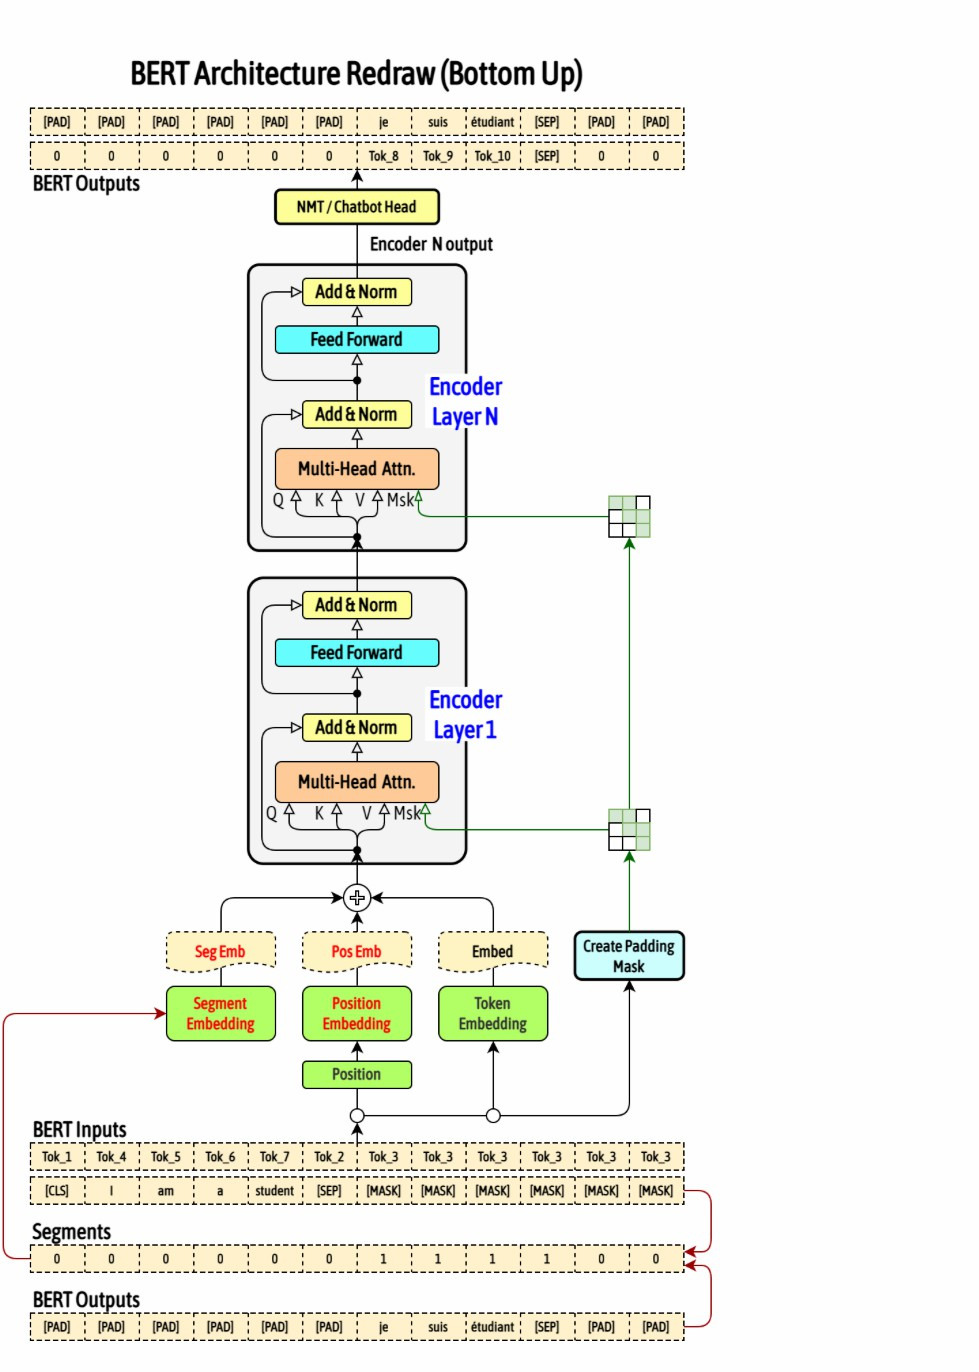
\includegraphics[width=90mm]{Figures/BERT.jpg}
\caption{BERT Architecture. Image sourced from \url{https://wikidocs.net/book/1}.\label{4}}
\end{figure}

\section{Tokenization}
BERT uses a WordPiece tokenizer to convert sentences into tokens. The main goals of tokenization are splitting words into subword units, handling out-of-vocabulary words, padding to ensure equal-length sequences, and adding special tokens \texttt{[CLS]} and \texttt{[SEP]}. As an example, the following words are converted into the following word pieces:

\begin{table}[H]
    \centering
    \begin{tabular}{|l|l|}
        \hline
        \textbf{Word} & \textbf{WordPiece Tokens} \\
        \hline
        running & [run, \#\#ing] \\
        happiness & [happi, \#\#ness] \\
        unreadable & [un, \#\#read, \#\#able] \\
        football & [foot, \#\#ball] \\
        unbelievable & [un, \#\#believ, \#\#able] \\
        \hline
    \end{tabular}
    \caption{WordPiece Tokenization}
    \label{tab:wordpiece}
\end{table}
In addition to separating each sentences into word piece token, word token that have not been seen previously will be set as \texttt{[UNK]}.

\section{Embedding Layer}
After tokenization, BERT converts each token into a high-dimensional vector using word embeddings. The embeddings are the sum of token embeddings, positional embeddings, and segmentation embeddings. The total embedding for each token is given as:
\begin{equation}\label{eqn11}
    \text{embedding}(i) = \text{token\_embedding}(i) \allowbreak + \text{position\_embedding}(i) \allowbreak + \text{segmentation\_embedding}(i)
\end{equation}

\section{Transformer Encoder Layer}
BERT is composed of 12 transformer encoder layers. Each layer integrates components such as multi-head self-attention, layer normalization, residual connections, and feed-forward networks (FFNs). The fundamental operation within the transformer is self-attention, which enables each token to consider the entire input sequence when generating its representation. In multi-head attention, the model employs \textit{n} parallel attention heads, each performing scaled dot-product attention independently. The outputs from these heads are then concatenated and passed through a linear transformation using a weight matrix \( W_o \):

\begin{equation}\label{eqn12}
    \text{MultiHead}(\text{h}) = [\text{Attention}_1(\text{h}),\dots,\text{Attention}_n(\text{h})] \text{W}_o
\end{equation}
After the computation of attention, BERT adds the original input to the attention output using a residual connection:
\begin{equation}\label{eqn13}
    \text{h}' = \text{LN}(\text{h} + \text{MultiHead}(\text{h}))
\end{equation}
\begin{equation}\label{eqn14}
    \text{SA}(h) = \text{FFN}(\text{h})
\end{equation}

where LN is layer normalization. Each encoder layer contains a feed-forward network that performs two linear transformations with a non-linear activation function applied in between:
%\begin{equation}\label{eqn15}
%    \text{FFN}(\text{h}) = \text{W}_2 \text{f} (\text{W}_1 \text{h} + \text{b}_1) + \text{b}_2
%\end{equation}
\begin{equation}\label{eqn15}
    \text{FFN}(\text{h}) = \text{W}_2 \, \text{f} (\text{W}_1 \text{h} + \text{b}_1) + \text{b}_2\footnote{FFN: Feed-Forward Network}
\end{equation}

where \textit{f(.)} is an non linearity, we use GeLU in BERT  rather than ReLU. The Gaussian Error Linear Unit (GeLU) and Rectified Linear Unit (ReLU) are both activation functions that are widely used in neural networks, but their differences in handling negative values make GeLU particularly effective in complex models like BERT  whereas ReLU, defined as ReLU(x)=max(0,x), outputs zero for all negative inputs, creating a strict boundary at zero. GeLU introduces a smooth, probabilistic transition for negative values near zero. This smoothness ensures GeLU avoids abrupt saturation, maintaining gradient flow even for inputs slightly below zero.

\section{Pre-training and Fine-tuning BERT Model}
One of the biggest challenges in language model training is to determine a prediction goal. A directional method that may restrict context learning is used by several models to predict the next word in a sequence. BERT uses two advanced methods of training to address this issue:
\begin{itemize}
    \item \textbf{Masked Language Model (MLM)}  
    The MLM task helps BERT understand words by using their surrounding context. During training, about 15\% of the words in each sentence are selected for masking:
    \begin{itemize}
        \item 80\% of these words are replaced with the special \texttt{[MASK]} token.
        \item 10\% are replaced with random words.
        \item 10\% stay the same.
    \end{itemize}
    BERT is then trained to guess the original word at each masked position using the other words in the sentence. A classifier layer on top of BERT predicts the correct word from the vocabulary. Since it only tries to guess the masked words, BERT becomes very good at understanding context in both directions.
    
    \item \textbf{Next Sentence Prediction (NSP)}  
    The NSP task helps BERT understand how sentences are related. In this task, BERT is given two sentences and must decide if the second sentence follows the first one in the original text. 
    \begin{itemize}
        \item 50\% of the time, the second sentence is correct.
        \item 50\% of the time, it is a random sentence from somewhere else.
    \end{itemize}
    To prepare the input:
    \begin{itemize}
        \item A \texttt{[CLS]} token is added at the start.
        \item A \texttt{[SEP]} token separates the two sentences.
        \item Segment embeddings mark which words belong to Sentence A or Sentence B.
        \item Positional embeddings encode the position of each token within the input sequence.

    \end{itemize}
    The output from the \texttt{[CLS]} token is passed through a small classifier that predicts whether the second sentence follows the first. A softmax function is used to give a probability.
\end{itemize}

\begin{equation}\label{eqn16}
    \text{Total Loss} = \text{NSP Loss} + \text{MLM Loss}
\end{equation}

\section{Fine-tuning for Downstream Tasks}
% BERT's flexibility allows it to be fine tuned on task specific data with minimal changes in architecture like  Text Classification which adds a classifcation layer on [CLS] token's output, Named Entity Recognition which uses token level embeddings also BERT is fine-tuned for question answering tasks, such as on the SQuAD dataset\cite{rajpurkar2016squad}, by training span prediction layers to predict the start and end positions of the answer span within a given context.
BERT's versatility enables it to be fine-tuned for various NLP tasks with minimal architectural modifications. For instance, in text classification, a classification head is added on top of the [CLS] token's representation. For named entity recognition (NER), BERT leverages token-level embeddings to make predictions. In question answering tasks like those based on the SQuAD dataset~\cite{rajpurkar2016squad}, BERT is fine-tuned by learning to identify the start and end indices of the answer span within the context.


% \textbf{What is the difference between pre-training and fine-tuning BERT?}  
% During pre-training, the model is trained on unlabeled data over different pre-training tasks. For fine-tuning, the BERT model is first initialized with the pre-trained parameters, and all of the parameters are fine-tuned using labeled data from the downstream tasks.

\textbf{What is the difference between pre-training and fine-tuning BERT?} \\
Pre-training involves training the model on large-scale unlabeled text using specific self-supervised objectives. In contrast, fine-tuning adapts the pre-trained BERT model to a specific task by updating all of its parameters using labeled data relevant to that task.
